\documentclass{article}

\usepackage{amsmath}
\usepackage{array}
\usepackage{authblk}	% prettier multiple authors
\usepackage[top=1in, left=1in, right=1in]{geometry}
\usepackage{graphicx}
\usepackage{hyperref}
\usepackage[group-separator={,}]{siunitx}
\usepackage{pdfpages}
\usepackage{tikz}
\usepackage{url}
\usepackage{xfrac}


% see http://texblog.org/2008/05/07/fwd-equal-cell-width-right-and-centre-aligned-content/
\newcolumntype{x}[1]{%
>{\centering\hspace{0pt}}p{#1}}%


\title{Unexpected Events In Social Data: The Social Media Pulse}
\author[]{Scott Hendrickson}
\author[]{Josh Montague}
\affil[]{Twitter, Inc.}

\begin{document}

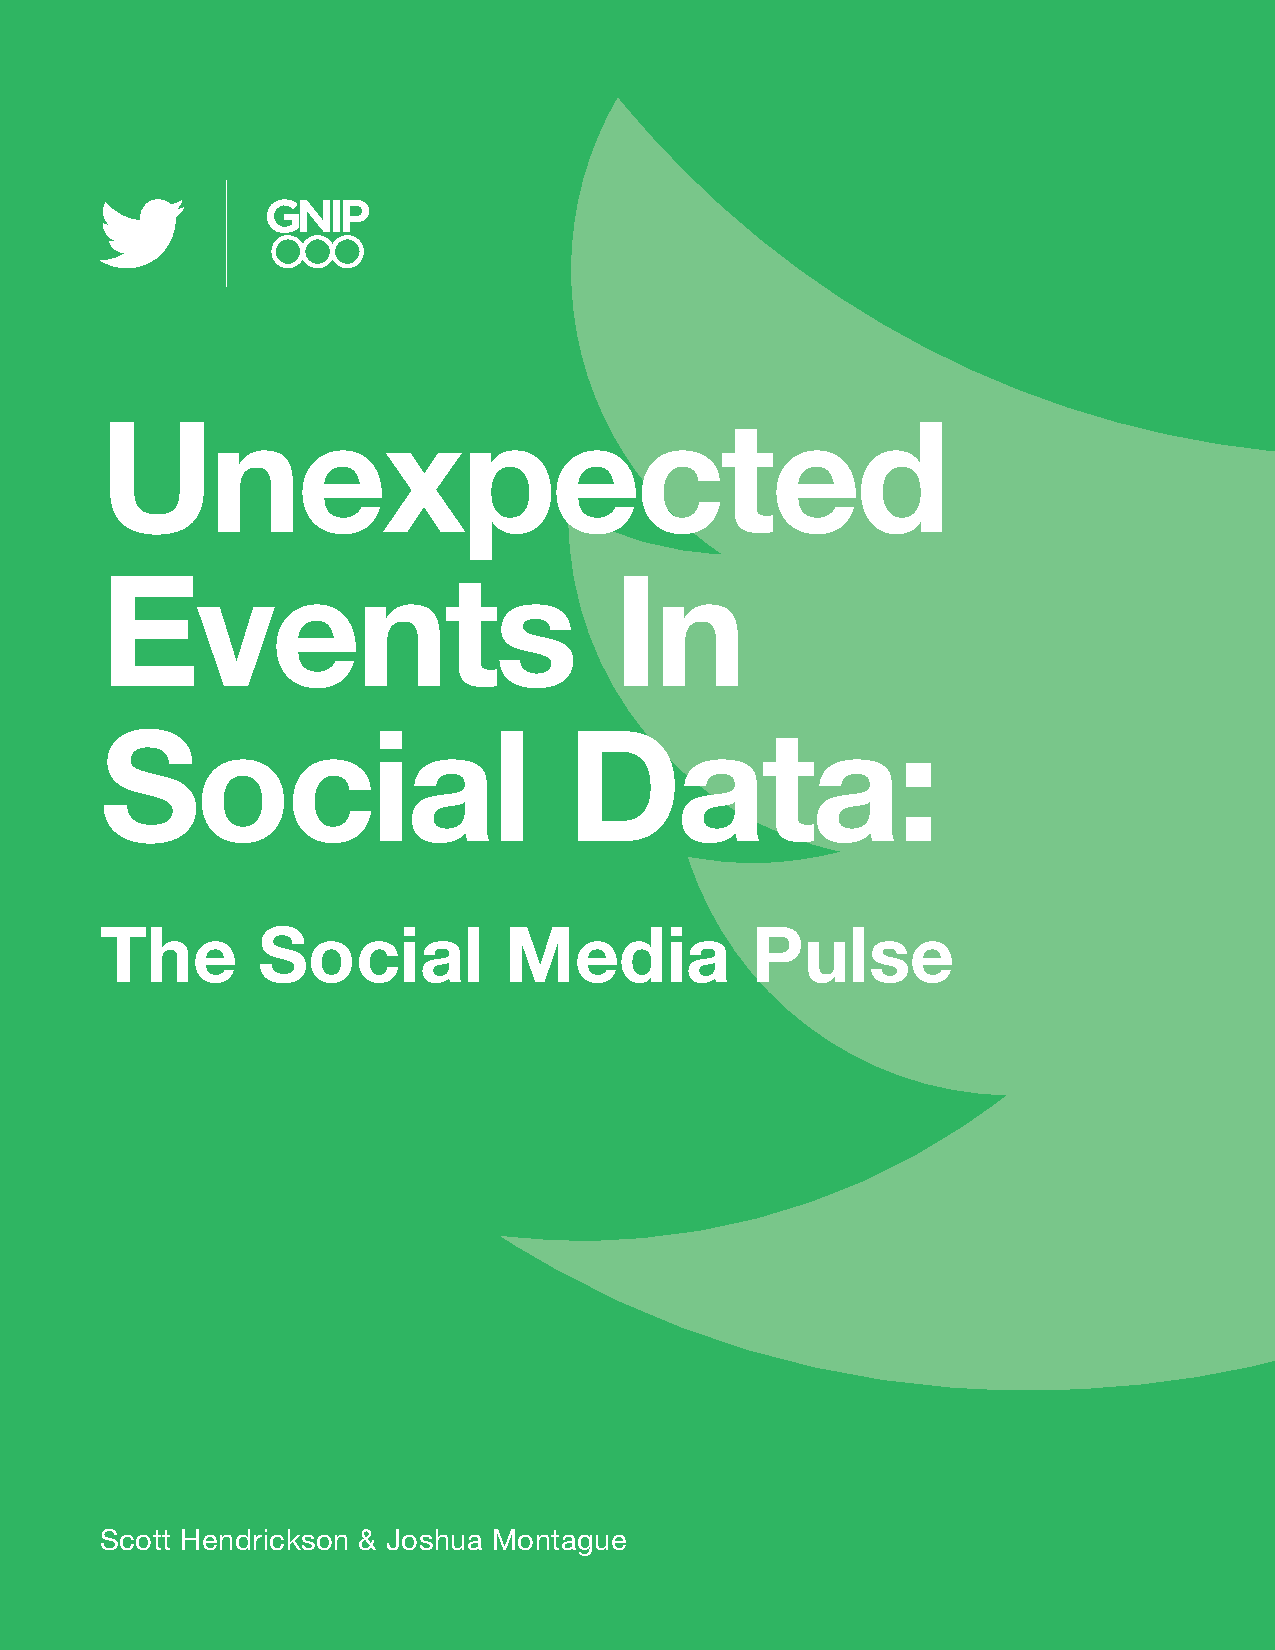
\includepdf[pages={-}]{front-cover.pdf} 
% no title if cover page
%\maketitle     

%%%%%%%%%%%%%%%%%%%%
\section{Introduction}
\label{sec:intro}

% context + motivation (experience => descrip/predictive models)
In the digitally connected world, social media platforms are often the primary means by which people share their observations and perspectives during significant events. Such platforms present low-friction ways to share their point-of-view experiences, whether in simple text or visual media (photos, videos, gifs, etc.). Because of this ease of sharing, the aggregate data produced by the platform's users is a rich source of insight into broad, cultural behavior. At times, we can even observe the ways by which these behaviors manifest in platform-specific patterns. Given enough data that displays these patterns, we can begin to develop models based on them.   

An analyst can be prepared to produce both descriptive and predictive results based on observed data by empowering them with models that describe the users and the users' responses to events. Obtaining a model representation of the data enables the analyst to compare parameters across multiple events (e.g., time scales, coefficient magnitudes); or, for a single event, one could compare similar parameters across multiple social platforms. Such a model could also be a component of broader trend- or event-detection methods, potentially assisting the analyst in handling real-time news media or public relations. 

In this article, we discuss three types of patterns that we have observed in Twitter data that relate to different kinds of events that manifest on the platform. We then discuss a quantitative model for one -- the Social Media Pulse. We present examples of each type of event, and an example of using the software that accompanies this paper to model the Social Media Pulse.\cite{pulse}


%%%%%%%%%%%%%%%%%%%%
\section{Event types}
\label{sec:models}

% expected vs. unexpected
Large events --- as classified by the volume of data generated by users of a social platform like Twitter --- can be thought of as either having been anticipated beforehand (expected), or not (unexpected). An example of an expected event is the arrival of a hurricane whose path toward land has been tracked by meteorologists over a number of days; an example of an unexpected event is an earthquake affecting a populated area. 

% unexpected flavors
In the time period immediately following an unexpected event, we often observe two different types of response in the corresponding social media data depending on the situation surrounding the event. In one case, consider an event such as an announcement involving a cultural celebrity. Such an announcement is often shared by one (or a small number of sources), initially observed by a potentially small number of users, and then shared -- virally -- through the network graph of the platform. The data related to this type of event is typically observed to begin with small volumes but quickly grow at an increasing rate before eventually saturating at a peak and decaying. 

In a second case, consider an event such as an earthquake, which is observed -- first-hand -- by some number of users who all subsequently reach for a device to share this news. This type of event, however, does not initially spread virally through the platform graph. While it may be re-shared and discussed by others to some extent, the primary source of data is from observers. As a result, the corresponding data typically pulses rapidly from nearly zero (or some low baseline) to a peak before gradually decaying back to the previous baseline. 

In this work, we refer to three types of events and their appearance in the associated data as: ``expected", ``unexpected network effect", and ``unexpected pulse" or ``Social Media Pulse" (SMP). 

In the remainder of this section, we briefly discuss the expected and unexpected network effect events, and then expand on the foundations of the SMP model. 


%%%%%%%%
\subsection{Expected event}
\label{sec:models_ex}

% mechanism for ~symmetric shape to expected event (human nature)
We refer to situations where an event has been forecasted or otherwise expected beforehand as an expected event. The pattern of these expected events is characterized by a gradual growth in activity rate over time. As the event draws closer -- and depending on the nature and severity of the impending event -- people naturally converse about plans or preparations for the event, or sometimes circulate jokes about the event. Similar conversations can occur after the event, where a kind of collective social debriefing occurs, sometimes involving additional popular stories, memes, or insights on the topic. The resulting shape of the data in these cases can (but does not have to) be somewhat symmetric around the event. The duration of the event -- some portion of the peak-width observed in the data -- may span hours or days depending on the nature of the event. If the event covers a sufficiently large timescale, the daily cycles of platform usage as a whole may be seen superposed on the data. 

% expected: winter storm jonas (Jan 2016)
An example dataset reflecting this type of expected event is shown in Figure \ref{fig:jonas}. In this Figure, the hourly activity rate (in count of Tweets per hour) discussing ``jonas" in the days preceding -- and following -- the winter storm in January of 2016. In the days leading up to the landfall of the storm (approximately 23 January), we observe a growing level of discussion which reaches a peak on 24 January, and then returning toward a baseline level (including non-storm related use of the term ``jonas"). 

% figure: jonas  
\begin{figure}[!b]
\centering
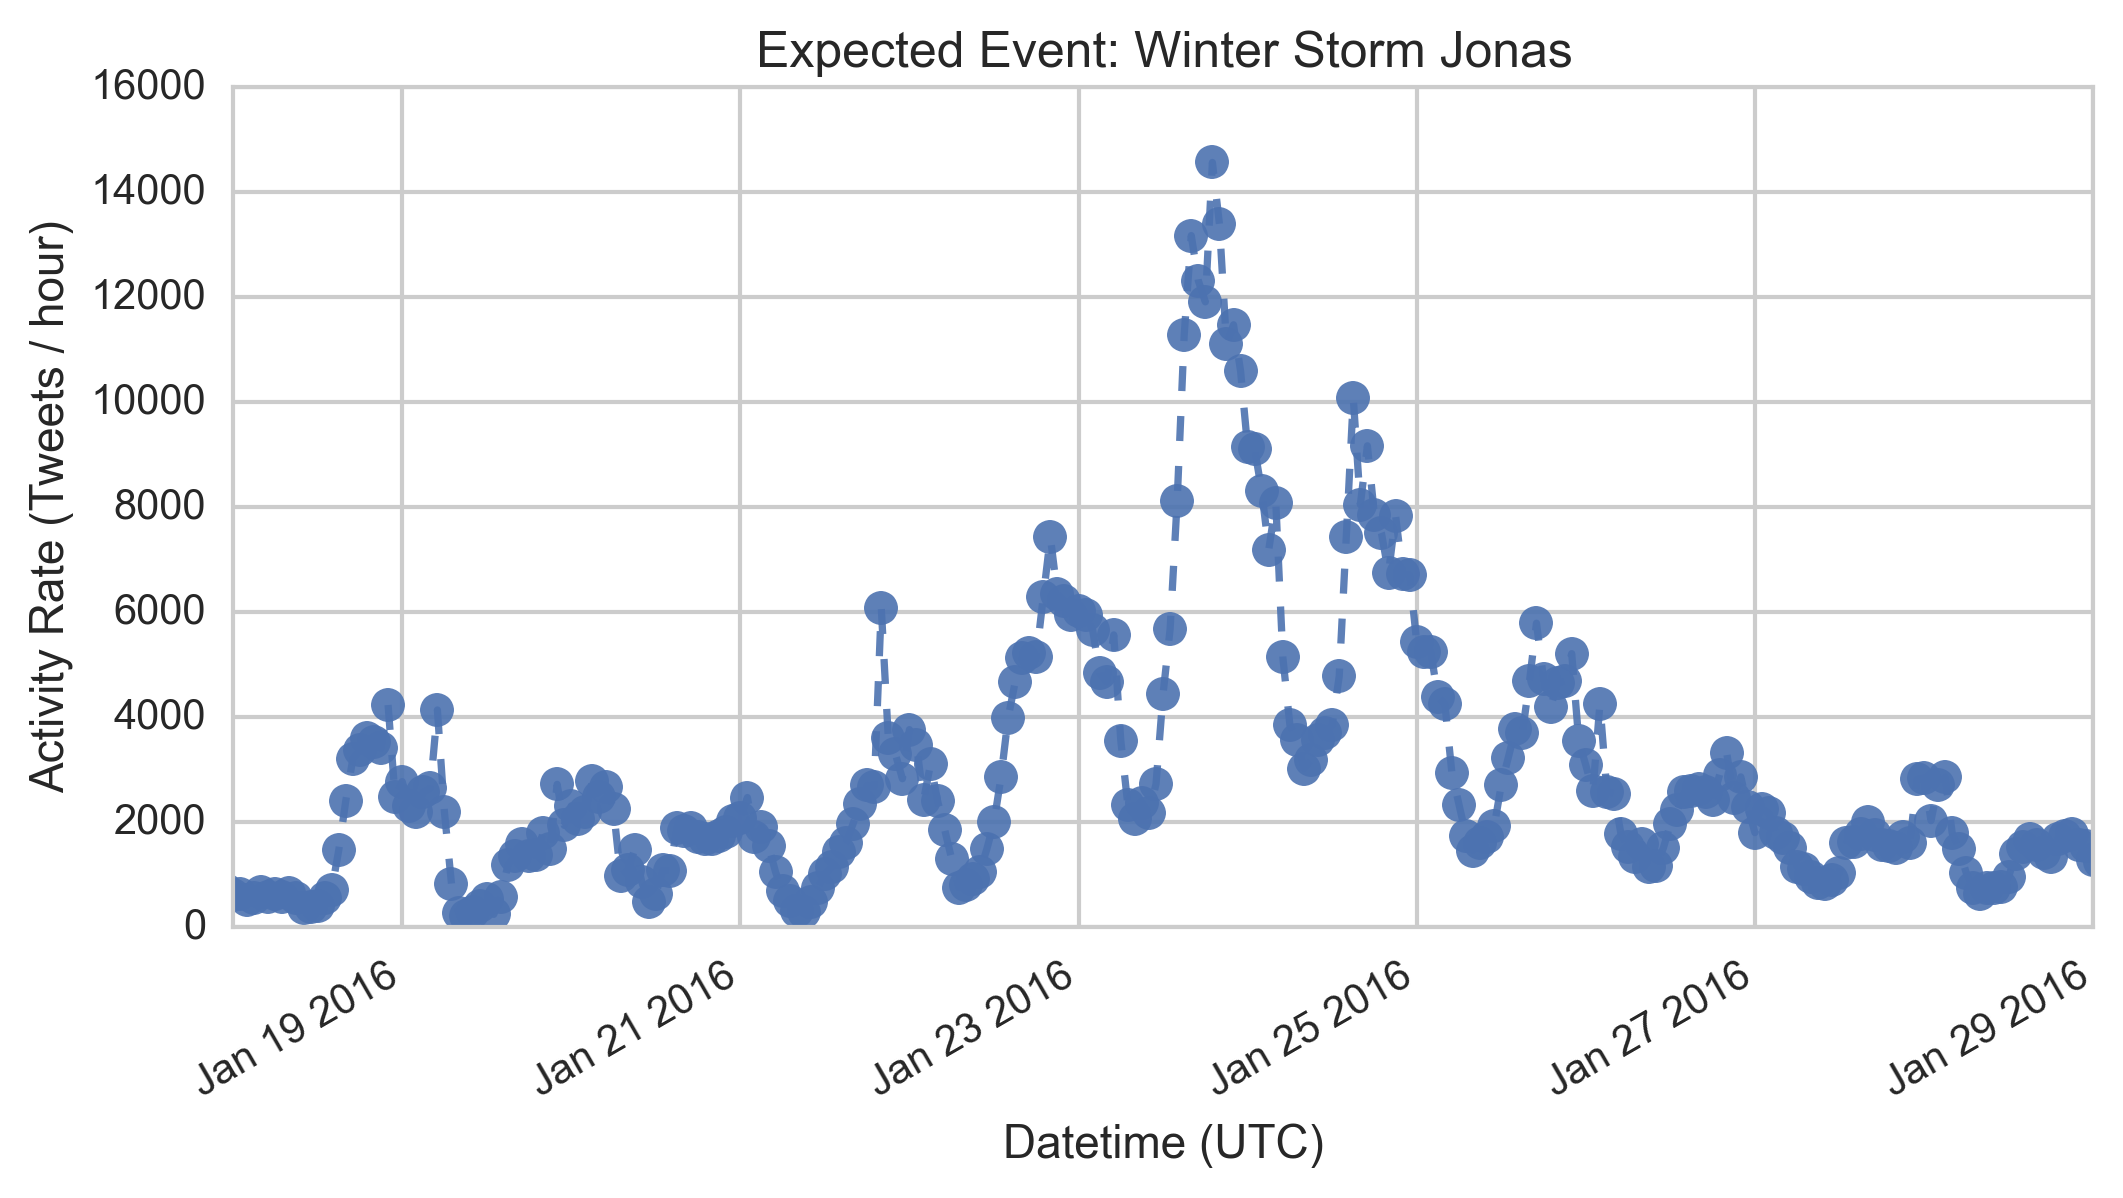
\includegraphics[width=0.9\textwidth]{img/jonas.png}
\caption{Conversation about ``jonas" in the period surrounding landfall of Winter Storm Jonas in January 2016. The hourly activity rate grows gradually to a peak around 24 January, and then decreases toward a lower baseline in the days following. This trend is superposed on the daily background cycles also visible in the data. Dashed lines connect the data points in the series.}
\label{fig:jonas}
\end{figure}


% other examples + asymmetry
Other examples of expected events include award shows, where the media make predictions about e.g. the fashion and award recipients ahead of time; the arrival of a national holiday, where people are discussing their plans; or an election, where all candidates make concerted marketing efforts to drive conversations about their party before the event. In many of these cases, the data corresponding to these topics has an asymmetry around the peak of activity. While it is tempting to speculate on how the specific asymmetry of these peaks might be driven by some set of cultural norms, expected events are observed to demonstrate greater rates of change on both the leading and trailing edge of their event peak. This remains an open area of research.  

%%%%%%%%
\subsection{Unexpected network spread}
\label{sec:models_unex-net}

% mechanism for unexpected network spread 
Events that are both unexpected and extensively shared through the social network graph are referred to as unexpected network spread events. During these types of events, the propagation of information about the event is by digital ``word of mouth" on the social media network, and there is a large number of users interested in resharing the content. After being shared on the platform by a source (or small group) the knowledge of this event spreads to additional users -- who were not present to report on the initial event -- purely by the connections of the network. In particular, the data generated by this type of event demonstrates an exponential growth in observed activity rate prior to peaking, and subsequently reducing in the wake of the news. In the case of Twitter this activity rate is driven by the observation of Tweets and Retweets from users on the platform that are not directly connected, but share a connection within the social graph. Due to the massive number of connections on the platform, this information can cascade and spread very quickly. 

An example of an event that was shared through the Twitter platform at this kind of increasing rate was the emergence of the unrest in Ferguson, Missouri, following the 2014 shooting death of Michael Brown.\cite{wiki:ferguson} As shown in Figure \ref{fig:ferguson}, the observed rate of conversation about ``ferguson" grew at an increasing rate for many days before reaching a single-day peak in the millions. As was reported by the Pew Research Center, awareness of the situation in Ferguson was spread primarily through Twitter before the cable news networks began discussing the events in the subsequent days.\cite{Hitlin2014} 

% figure: ferguson
\begin{figure}[!b]
\centering
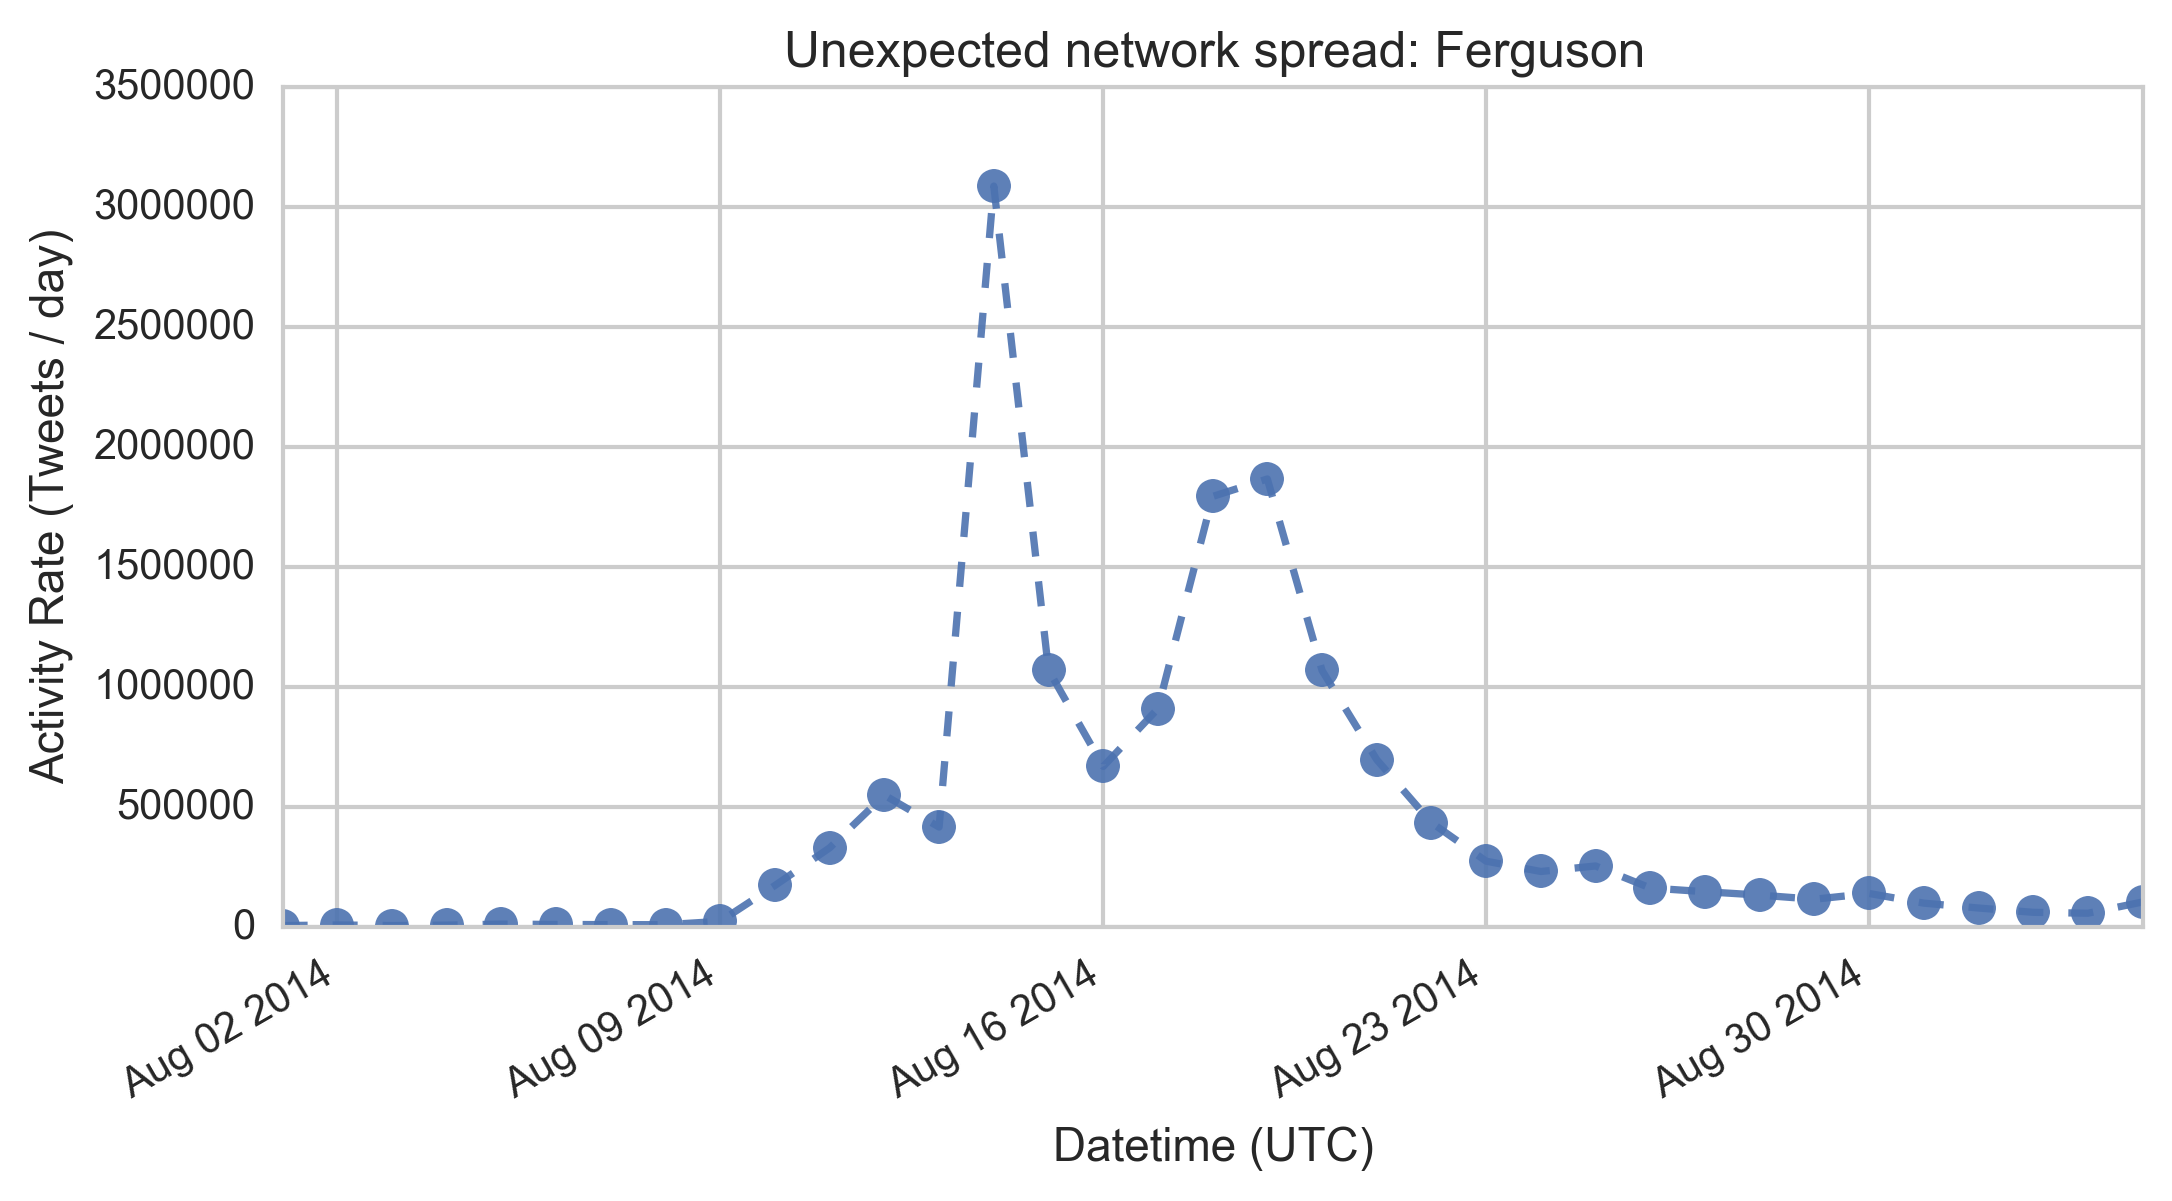
\includegraphics[width=0.9\textwidth]{img/ferguson.png}
\caption{Conversation about ``ferguson" in the weeks surrounding the shooting death of Michael Brown and subsequent unrest in Ferguson, Missouri. For many days, the observed daily activity rate grew until peaking near 14 August 2014. The exponential growth in activity rate is a result of the broad propagation of information through the Twitter social network graph. Dashed lines connect the data points in the series.}
\label{fig:ferguson}
\end{figure}

% refs on network effects 
Though this type of network spread is an interesting topic, we do not propose a robust model for it in this work. Building operational systems around this type of event can be challenging; small, relevant, early signals of viral events can be buried beneath high-noise data, particularly in any realm where there is significant speculation. As a result, additional, customized, possibly domain-specific techniques are required to boost the signal-to-noise ratio in these domains. More generally, there is an active field of research in the theories of information diffusion and virality within social networks.\cite{Gruhl2004,Weng2013,BosaghZadeh2013,Ferrara2015} 


%%%%%%%%
\subsection{Unexpected pulse: Social Media Pulse}
\label{sec:models_unex-pulse}


% mechanism for SMP
Events that are both unexpected and simultaneously witnessed and shared by many observers can be considered to be of the Social Media Pulse (SMP) type. During such an event, we ascribe the majority of generated data to the immediate observers of the event. In the immediate wake of their observations, these users reach for a mobile phone or computer to share their experience and observation. As a result of this process, the shape of these events in time is typically a very sharp rise in activity rate, followed by an exponential decay. 

% example: robin williams
An example SMP is shown in Figure \ref{fig:williams}, where the normally low-volume background of conversation on ``robin williams" increases abruptly following the breaking news of the actor's death on 11 August 2014. The news broke from a handful of news-related Twitter accounts and was subsequently observed, nearly simultaneously, by hundreds of thousands of their followers. Following this abrupt spike, the activity rate drops off exponentially.  


\begin{figure}[!b]
\centering
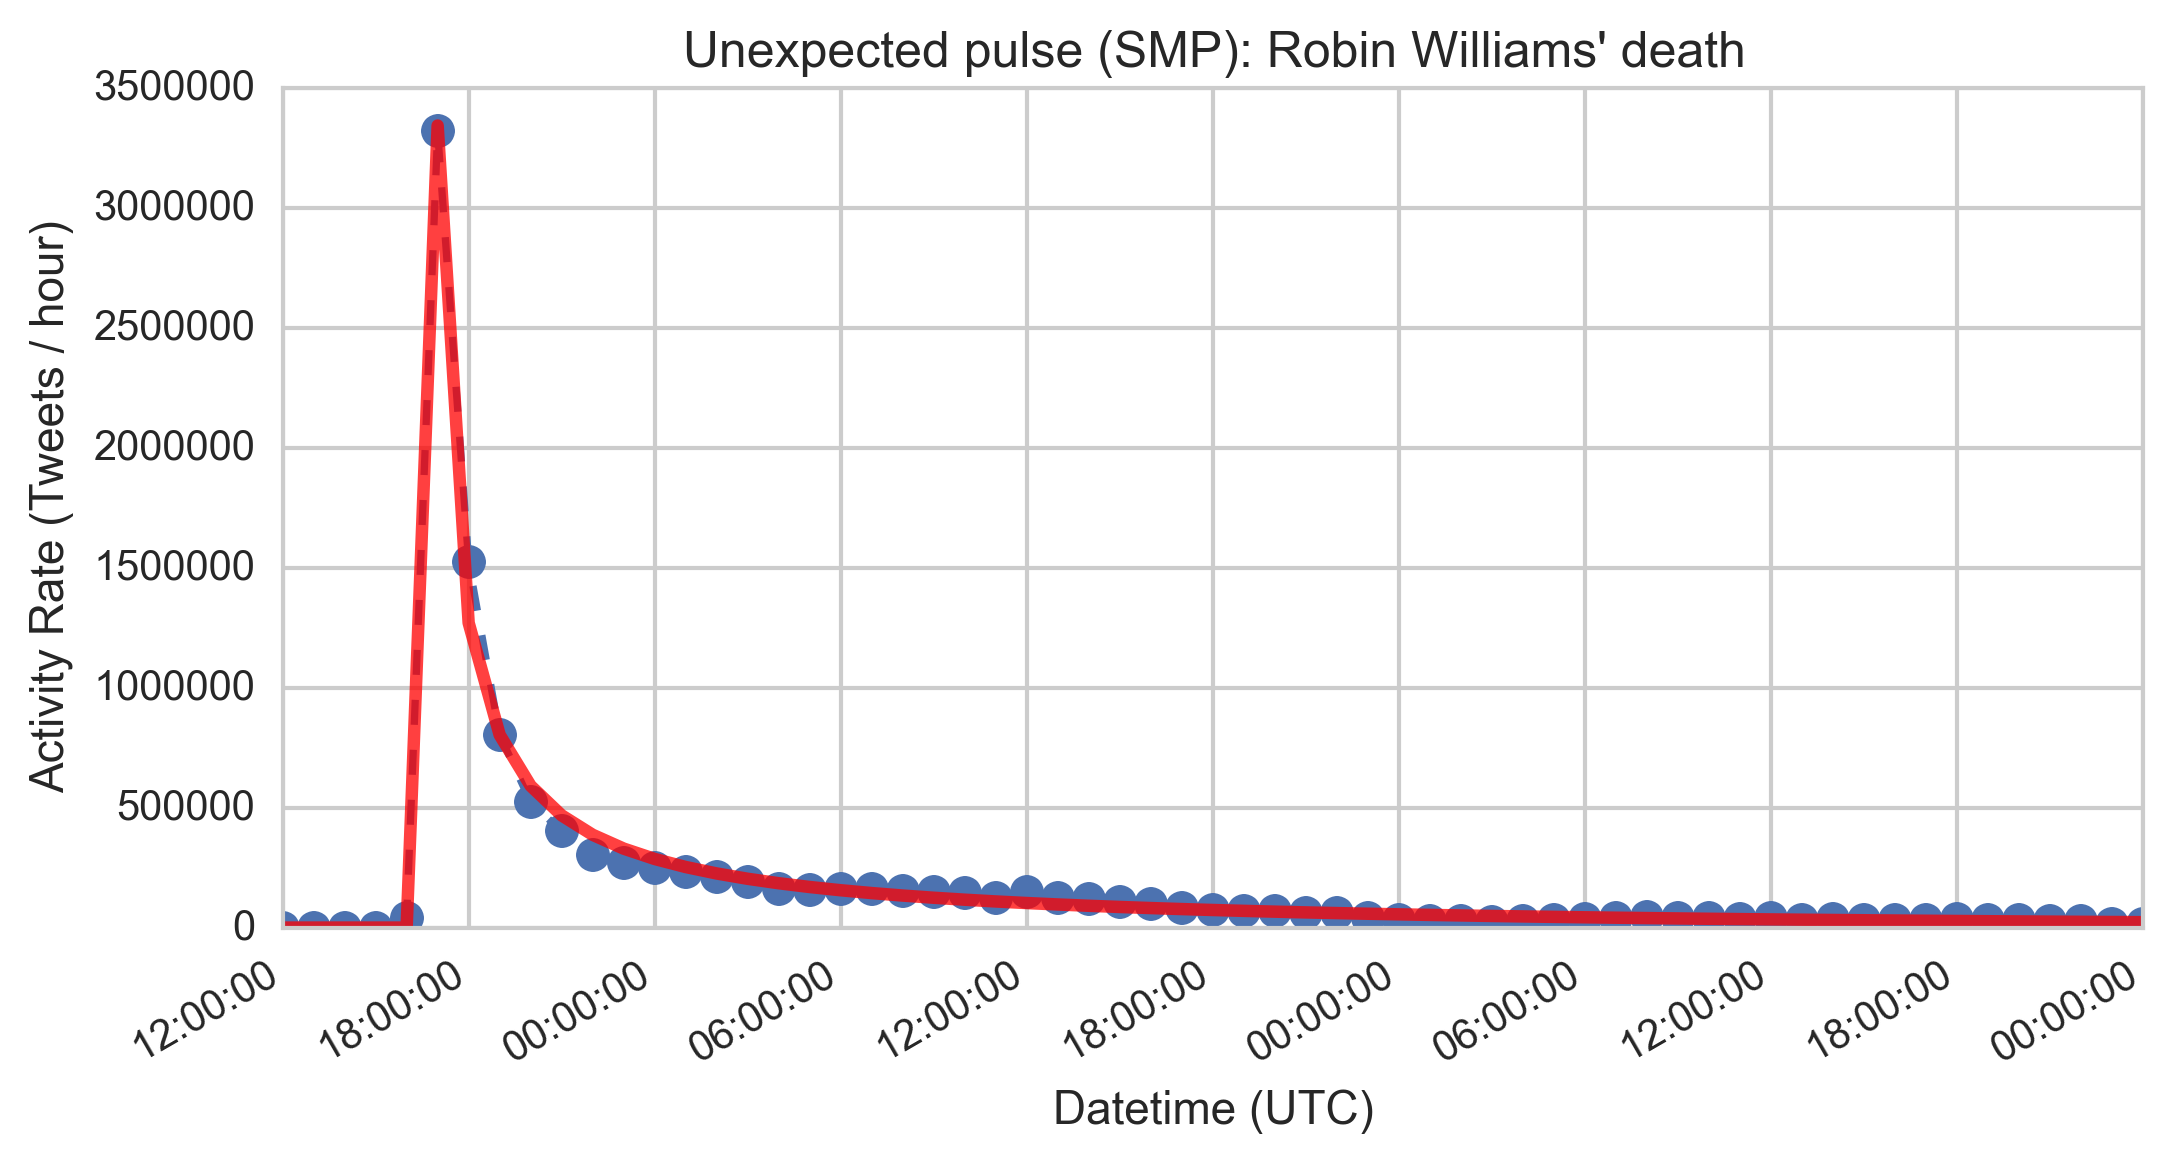
\includegraphics[width=0.9\textwidth]{img/williams.png}
\caption{Conversation around ``robin williams" in the hours surrounding the breaking news of his death on 11 August 2014. The news broke from a handful of news-related Twitter accounts and was subsequently observed, nearly simultaneously, by hundreds of thousands of their followers. The abrupt rise in activity counts, followed by a decay toward a lower background level is typical of the SMP model. The solid line is an SMP model fit to the data, discussed in Section \ref{sec:models_unex-pulse}. Dashed lines connect the data points in the series.}
\label{fig:williams}
\end{figure}


% stat model
The SMP describes a Poisson counting process, and we assume that the underlying probability of the time to Tweet for any one user follows an exponential distribution. There are many references available to learn more about the statistics behind this particular type of model,\cite{wiki:poisson} but we will briefly cover some of the motivation here. Following the unexpected event, the probability of an observer posting on the topic at time $t$ decays with a constant rate parameter $\lambda$ such that

% exponential probability distribution
\begin{equation}
f(t;\lambda) = \lambda e^{-\lambda t}, \text{ for } t \geq 0.
\label{eq:exponential}
\end{equation}
Here, we have allowed the time $t$ between the event ($t=0$) and the Tweet to be our independent random variable $X$, where $X \sim Exp(\lambda)$. Hypothetically, if the same person were to observe the same event multiple times and Tweet about it, the expected value of their time to post is given by the expected value of the distribution (mean, or first moment) $E(X)=1/\lambda$.

% convolution of Exps => Gamma
On a social platform, we are looking at the aggregate activity of many observers. In this case, we will make the following assumptions: the rate parameter associated with any one individual will be the same, and the value of $t$ for an individual will be independent of any other. That is, we have a new random variable that is the sum of many of the $X$s above, $S = X_1 + X_2 + \ldots + X_n$. The convolution of a set of individual exponential distributions gives the gamma distribution.\cite{Hogg2013} As a result, to calculate the probability of Tweeting at time $t$ for this new random variable, we start with the probability density function for the gamma distribution: 

% gamma distribution, pdf
\begin{equation}
f_S(t;\alpha,\beta) = \frac{ \beta^{\alpha} } {\Gamma(\alpha) } (t-t_0)^{\alpha-1} e^{-\beta(t-t_0)}, 
\label{eq:gamma}
\end{equation}
which is defined in terms of a shape parameter $\alpha$, a scale parameter $\beta$, and the gamma function $\Gamma(\alpha)$.\cite{Hogg2013} We also include an allowance for the start of the pulse to vary from the first observed data point as $t_0$. Note that the shape parameter $\alpha$ is unitless, while the scale parameter $\beta$ takes on units of $1/[X] = t^{-1}$. To project the gamma distribution model onto observed data, we will also include a multiplicative constant $a_0$ in the formula which will take on the same rate units as the input data eg. activities per unit time. We will later use these model parameters to compare events. It is worth noting that the gamma distribution can be written with other parametrizations. Another common variation is given in terms of shape parameter $k = \alpha$ and scale parameter $\theta = 1/\beta$. 

With the probability distribution $f_S(t;\alpha,\beta)$, we can think about the activity rate estimate over any timeframe $t_f - t_i$ as

% rate estimate
\begin{equation}
r(t) = \frac{ N_{act} }{ t_f - t_i } \int_{t_i}^{t_f} f_S(t) dt, 
\label{eq:gamma-rate}
\end{equation}
where $N_{act}$ is interpreted as the total number of activities observed -- due to the pulse model alone -- from $t = 0$ to $t \rightarrow \infty$. In Section \ref{sec:pulse-deviations}, we will discuss how this count can -- at times -- underestimate the actual observed number of activities. With the probability distribution given in Equation \ref{eq:gamma}, and the calculated rate estimate from Equation \ref{eq:gamma-rate}, we are nearly prepared to fit time-series data associated with an event. As we will see in Section \ref{sec:smp-example} (and as is reflected in the model code \cite{pulse}), there will also be an overall normalization factor.  

The Twitter data with which we are concerned comprises a large number of individual Tweets, each containing a timestamp indicating the second at which it was shared. To transform from timestamped data to a time-series we will aggregate the count of activities within a time bin of duration $\delta t_{bin}$. This gives a ratio of activity count per time that represents the estimated activity rate over that period of time (bin). The quality of the model rate estimate depends on the relationship between the bin size and the timescale of the SMP $\delta t_{rise} = t_{peak} - t_0$, where $t_{peak}$ is the time corresponding to the maximum value of the activity rate. Ideally, $\delta t_{bin} \ll \delta t_{rise}$. In practice, it is often adequate to have $\delta t_{rise}$ only a few times $\delta t_{bin}$. And since estimates of averages vary as $\sim 1/\sqrt{ \text{sample size} }$, ideally we also choose $\delta t_{bin}$ such that the activity rate estimate is $\gg$ 1 activity per bin in the region of interest. 

Once we fit this model to a data set, we can use the resulting fit parameters to calculate additional metrics that describe the event and allow for comparisons between events. Below, we include a collection of such example metrics. 

\begin{enumerate}

%%%%%%  rise time  %%%%%%%

\item{ \textbf{Rise Time (Time-to-Peak)} } 
The rise time (or time-to-peak) $\delta t_{rise} = t_{peak} - t_0$ is the time duration between the start of the pulse and the maximum rate estimate. This is derived by maximizing Equation \ref{eq:gamma} and is given by:
\begin{equation}
\delta t_{rise} = \frac{ \alpha - 1 } { \beta } 
\label{eq:rise}
\end{equation}

This parametrization is also consistent with the mode of the Gamma distribution.\cite{wiki:gamma} 


%%%%%%  response time  %%%%%%%

\item{ \textbf{Balanced Response Time} }  
The SMP model often covers a wide window of time. The ``balanced response time" is meant to represent a balance point between the activity volume in the tall head of the pulse and long tail after the event. The balanced response time is given by

\begin{equation}
t_{bal} = t_0 + \frac{\alpha}{\beta}
\label{eq:bal}
\end{equation}

This parametrization is also consistent with the mean of the Gamma distribution.\cite{wiki:gamma} 


%%%%%%  total event volume  %%%%%%%

\item{ \textbf{Event Activity Volume} } 
The total activity volume for an event is the integral of the activity rate over time. Or, similarly, since our data collection is always over finite time intervals, a sum of activity rates. For some events the model will match the time-series well from $t_0$ to the end. In some cases, the time-series data will deviate from the model; in Section \ref{sec:pulse-deviations} we discuss such secondary sources as delayed news coverage of an event. In these circumstances, we consider the total event activity volume to be the count of activities that would have been measured had this secondary source not been present. The total count of activities is given by the time integral of the modeled activity rate: 

\begin{equation}
N_{act} = \int_{t_0}^\infty r(t) dt 
\label{eq:total-acs}
\end{equation}

\end{enumerate}


These parameters are calculated and reported by the software that accompanies this document.\cite{pulse} The fitting routine and calculations are written in Python and make use of the numerical libraries \texttt{SciPy} and \texttt{NumPy}.\cite{Jones} In Section \ref{sec:smp-example} we demonstrate an example of using this software on a real event. 




%%%%%%%%%%%%%%%%%%%%
\section{Example}
\label{sec:smp-example}

% examples of fits & discussion 
In this Section, we apply the SMP model to an example dataset to illustrate the process. The source code and example data, respectively, are available in the \texttt{src/} and \texttt{src/data/} directories of the associated GitHub repository.\cite{pulse} The initial release of this software is intended for command-line usage. It is designed with an expectation for input data in the form of a time-series CSV. Though other columns may be present, a timestamp column and count column must be present. The timestamp can either be in epoch seconds or ISO 8601-format datetimes,\cite{wiki:iso} such as delivered by the Twitter and Gnip APIs. In particular, the Gnip Search API \texttt{/search/counts} endpoint returns binned time-series data which is very compatible with this code. The SMP fitting code is written in Python and has some dependencies on packages outside of the standard distribution, namely \texttt{numpy} and \texttt{scipy}. Some Python distributions e.g. Anaconda\cite{anaconda} include these libraries. If you need to install them yourself, both can be installed with \texttt{pip}, the Python package manager. 

To see all available command-line flags that we can use with this tool, invoke the \texttt{smp.py} utility from the \texttt{src} directory with the \texttt{-h} option:

\begin{verbatim}
shell> ./smp.py -h
Usage: smp.py [options]

Options:
  -h, --help            show this help message and exit
  -i I_COL, --column-independent=I_COL
                        Column of independent variable for fit, 1-based count
                        (default: 1)
  -d D_COL, --column-dependent=D_COL
                        Column of dependent variable for fit, 1-based count
                        (default: 2)
  -p INIT_PARAMETERS, --init-parameters=INIT_PARAMETERS
                        Initial guess of model function parameters [x0, alpha,
                        beta, a0, y0]. If none are given, initial values are
                        calculated from input data (default: none)
  -w WINDOW, --fitting-window=WINDOW
                        Define a window of 0-1-scaled x values over which to
                        fit the curve e.g. '[0.1,0.7]'. If not given, entire
                        input range is used (not recommended). (default: none)
  -t, --real-time       Return output with time data in actual time [epoch
                        seconds, instead of 0-1 scaled] (default: False) 
\end{verbatim}

% simple example, no options
For a simple example of using this code, there is a comma-separated file of activity count data within the \texttt{/src/data/} called \texttt{test.csv}. If we make a chart of this data (with the time column as the independent variable), we observe a clear spike in the timeline. To apply our SMP model to this data from within the \texttt{src/} directory, we can pass the file contents to the utility either as an argument to the utility, or using the shell buffer: 

\begin{verbatim}
# for a simple, two-column data file... 
shell> ./smp.py data/test.csv 
# or, equivalently
shell> cat data/test.csv | ./smp.py 
# ... csv output (to shell stdout)...
# ... model parameters (to shell stderr)...
\end{verbatim}

% output format
The output of the utility is a three-column csv where the first two columns comprise the input data and the third column is the model fit, evaluated at each of the input points. This output is sent to the shell standard output stream. Following this output, the resulting model parameters and derived parameters are also displayed. This output is sent to the shell standard error stream. The example fit output data is shown in Figure \ref{fig:fit-pulse}, and the model and derived parameters are included in Table \ref{tab:unex-pulse}

% fit for meteor data
\begin{figure}[!h]
\centering
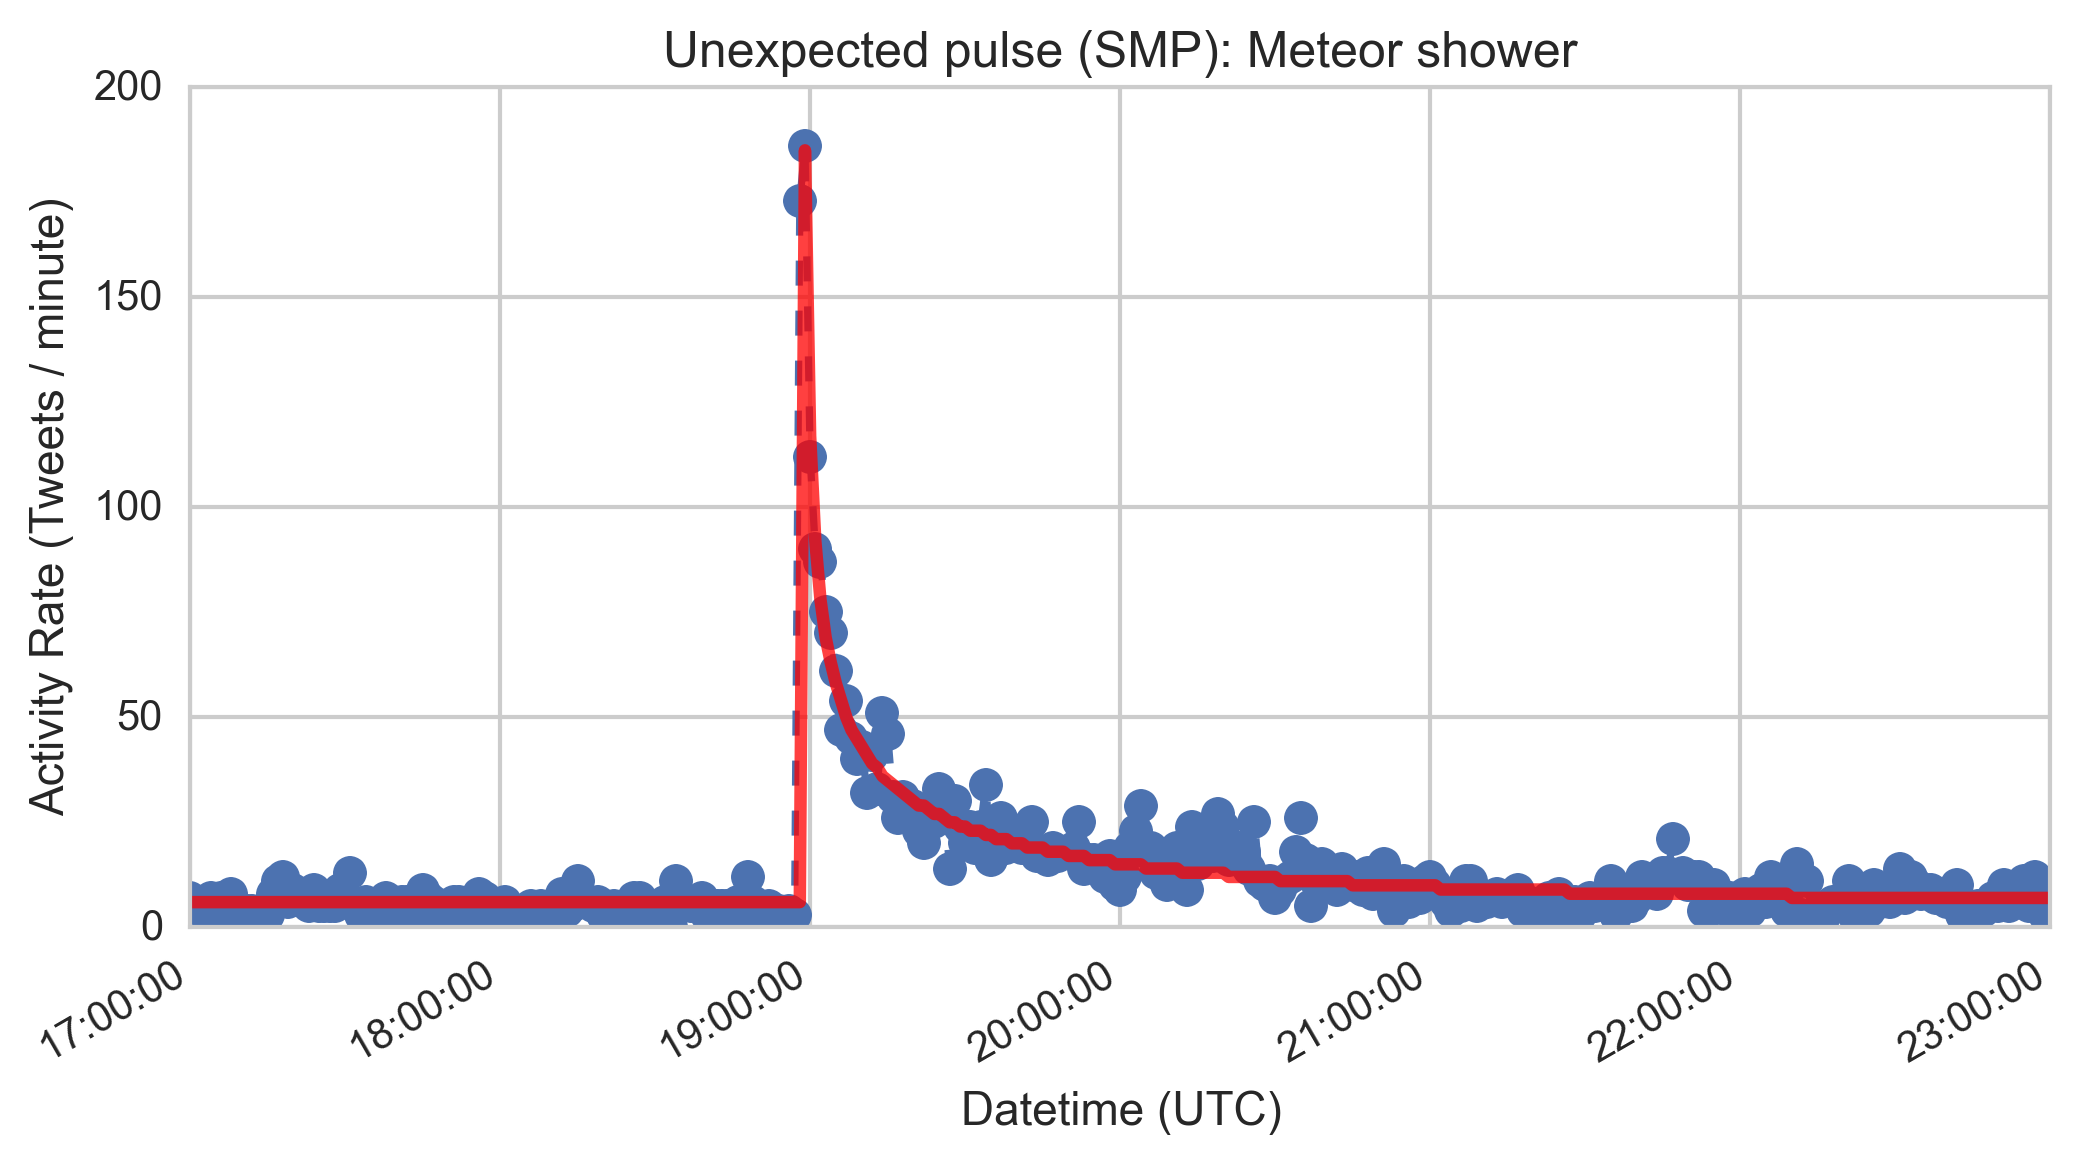
\includegraphics[width=0.9\textwidth]{img/meteor-shower.png}
\caption{Conversation around ``meteor" during a 2014 meteor shower. The solid line is an SMP model fit to the data. The resulting fit parameters are reported in Table \ref{tab:unex-pulse}. Dashed lines connect the data points in the series.}
\label{fig:fit-pulse}
\end{figure}


% table of parameters for the meteor fit
\begin{table}[!h]   % placement: h(ere), b(ottom), t(op), p(age, new), !(i mean it)
\centering
\begin{tabular}{ p{2cm} | p{2cm} }
\hline
Parameter       & Value     \tabularnewline     \hline
$a_0$           & 0.0216    \tabularnewline     \hline 
$t_0$           & 0.2982    \tabularnewline     \hline 
$\alpha$        & 0.4867    \tabularnewline     \hline 
$\beta$         & 6.4975    \tabularnewline     \hline 
$y_0$           & 0.0364    \tabularnewline     \hline 
\hline
$t_{bal}$       & 0.3731      \tabularnewline     \hline 
$\delta t_{rise}$   & 0.0     \tabularnewline     \hline 
$N_{act}$           & 1988    \tabularnewline     \hline 

\end{tabular}
\caption{Summary of fit parameters for the example Social Media Pulse model fit shown in Figure \ref{fig:fit-pulse}. By default, fit parameters and derived outputs are displayed in normalized units (both time and activity count normalized to 0-1 range). In the shell output, the rescaled values are also shown. $\delta t_{rise}$ is reported as zero when the modeled peak precedes the onset of the SMP.} 
\label{tab:unex-pulse}
\end{table}


% using the command line options 
As seen when using the \texttt{-h} option, there are command-line options for the utility which provide additional flexibility and functionality: 

\begin{itemize}  
\item The \texttt{-i} and \texttt{-d} options allow the user to specify custom column positions for, respectively, the independent and dependent data in the model. This is useful if the input CSV has additional data columns. 
\item The \texttt{-p} option allows the user to initialize the model with a custom set of parameters. When this option is not specified, a best guess is calculated from the input data. 
\item The \texttt{-w} option accepts a window (over the independent variable) over which the model parameter optimization is applied.
\end{itemize}

The SMP model fit convergence can overfit to data in the long tails (in part because the sum of squares error is additive), and so the \texttt{-w} option is particularly useful for limiting the region over which the fitting algorithm applies. The default independent output is in the scaled fit space (range of zero to one), such that the user can inspect the fit quality and experiment with the \texttt{-w} option values whose units are also in the scaled space. 

 


%%%%%%%%%%%%%%%%
\section{Comparison of SMP events}
\label{sec:pulse-comparison}

% compare multiple SMPs 
In Figure \ref{fig:smp-fit-comparison}, the activity rates associated with three separate earthquakes from April 2016 are shown. The collected data series are shown normalized to the range zero to one in both time and activity rate. The overlayed solid curves are SMP model fits to each series - each fit slightly different. Table \ref{tab:pulse-comparison} compares the resulting derived parameter values. The model variations afforded by the gamma distribution are seen in the shapes of both the leading edges and the trailing tails.  

These particular events happen to be relatively small in overall activity volume, leading to more variance in the observed data from the model fit. Nevertheless, the SMP model fit captures the overall behavior of the response to the sudden event. 


% quake comparison figure
\begin{figure}[!h]
\centering
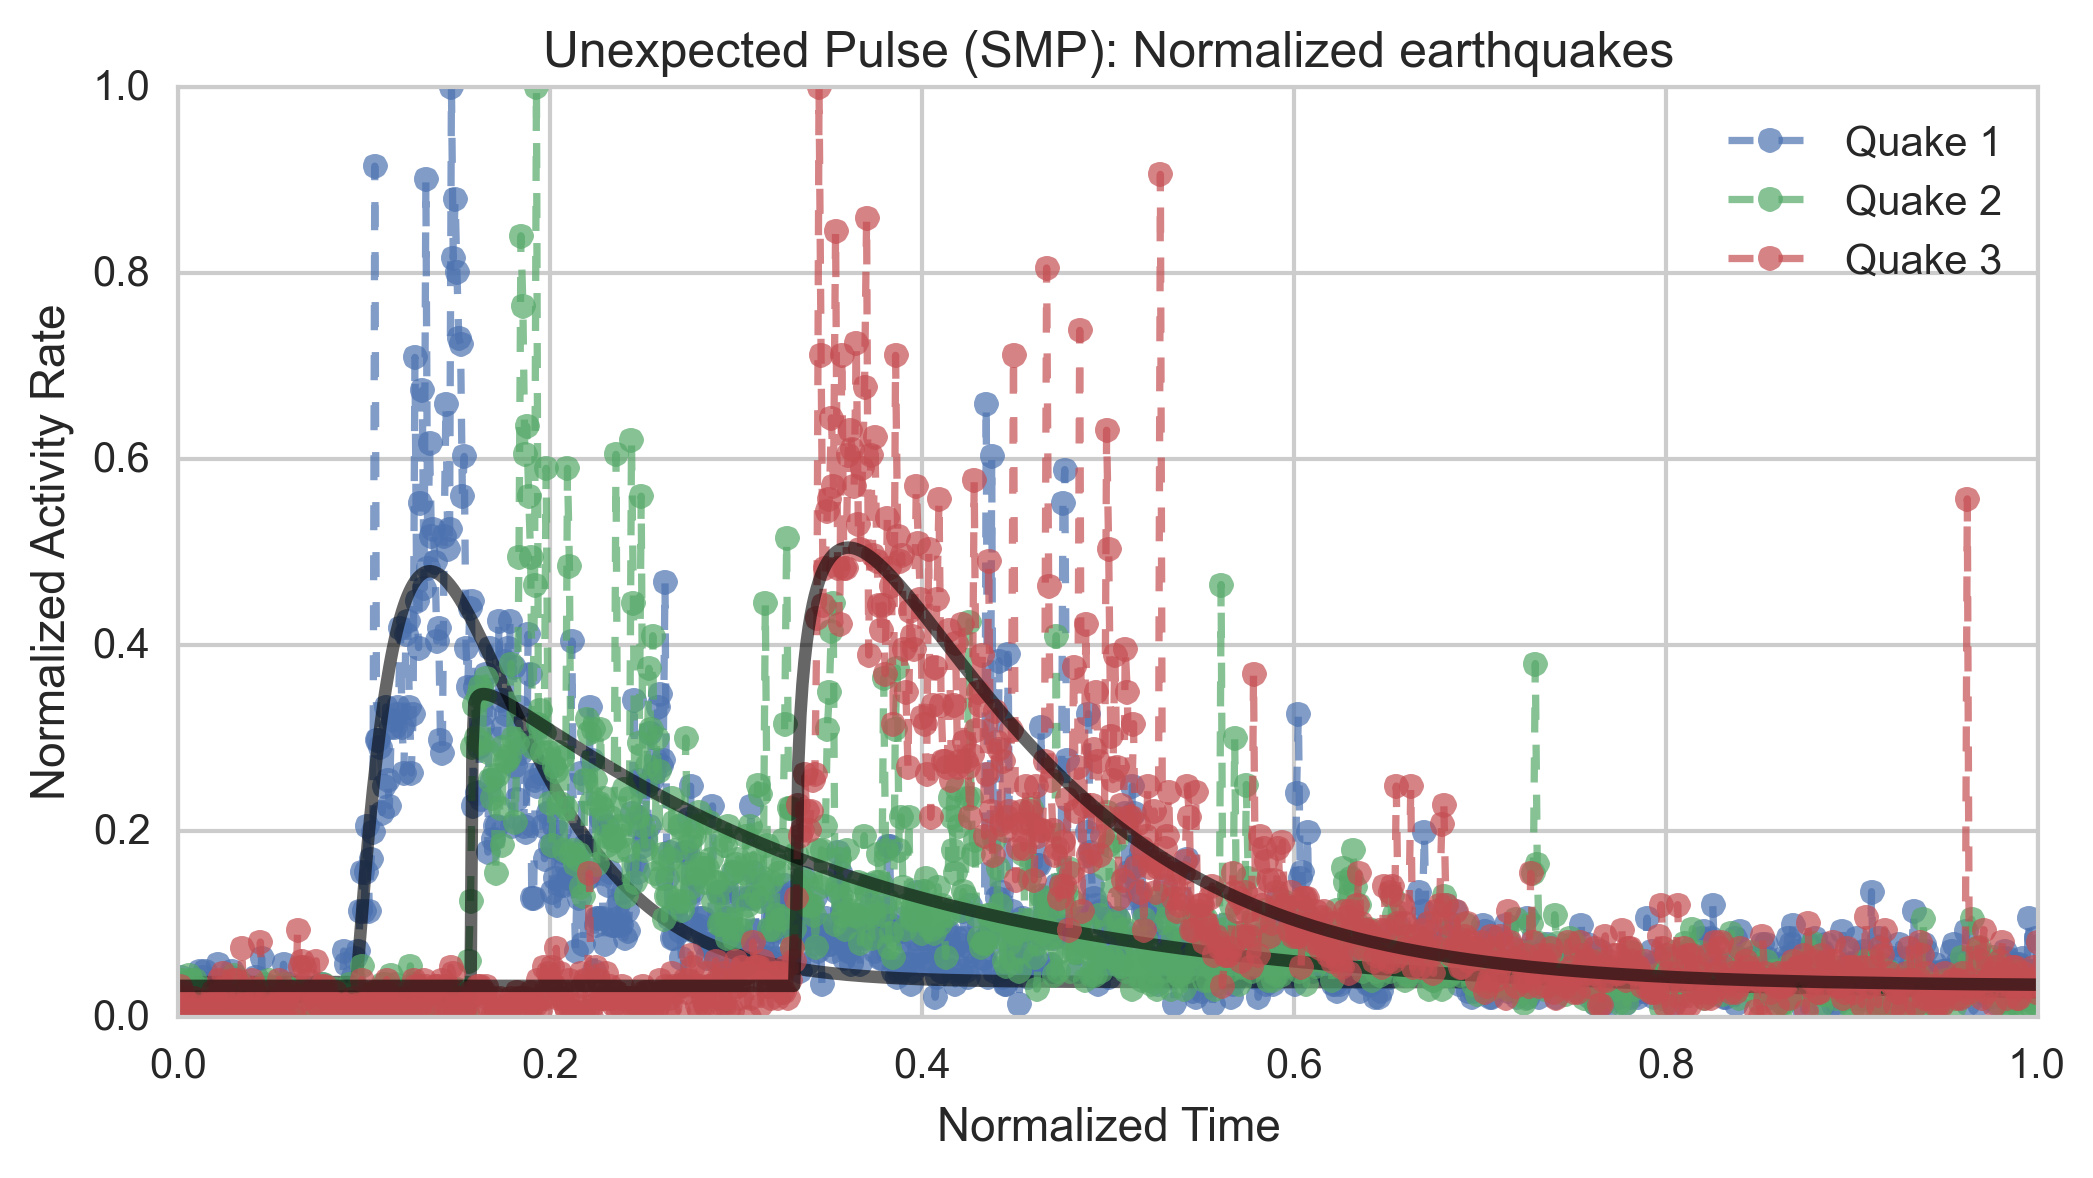
\includegraphics[width=0.9\textwidth]{img/compare-quakes.png}
\caption{A series of overlayed data series illustrating the normalized activity rate (activity counts and time both scaled to a range of 0 to 1) occurring in response to three earthquakes occurring in April 2016. Lower overall activity rates lead to noisier data. For each colored series, the solid black line overlayed illustrates an SMP model fit. Dashed lines connect the data points in each series.} 
\label{fig:smp-fit-comparison}
\end{figure}

% table of fit parameter comparison
\begin{table}[!h]
\centering
\begin{tabular}{ p{2cm} | p{2cm} | p{2cm} | p{2cm} }
\hline
        & $t_{bal}$ & $\delta t_{rise}$ & $N_{act}$ \tabularnewline     \hline
Quake 1 & 0.1727    & 0.0394            & 8492      \tabularnewline     \hline
Quake 2 & 0.3550    & 0.0059            & 18712     \tabularnewline     \hline
Quake 3 & 0.4537    & 0.0280            & 13488     \tabularnewline     \hline
\end{tabular}
\caption{Comparison of the derived parameters (normalized) from SMP model fits to three separate earthquake events. The corresponding data is shown in Figure \ref{fig:smp-fit-comparison}, on normalized axes. These values are described in Section \ref{sec:models_unex-pulse}, and presented by the command-line utility described in Section \ref{sec:smp-example}.} 
\label{tab:pulse-comparison}
\end{table}




%%%%%%%%%%%%%%%%
\section{Deviations from the SMP model}
\label{sec:pulse-deviations}

% example of data diverging from smp model 
In some circumstances, the decay observed after the peak of a SMP is interrupted by a change in the observed activity rate that does not follow the SMP model. These occasions can present unique opportunities to discover subsequent events in the data. In Figure \ref{fig:smp-fit-deviation}, we show an example of a set of data that was filtered on ``quake" in the vicinity of an actual earthquake. 

Generally, the data appears to be reasonably described by the SMP model. But, as indicated in the figure, there are notable points at which the activity rate deviates from the exponential decay predicted by the model, alone. In cases like these, we can use the specified time window to look at the Tweets being counted during these windows and frequently observe an increase in the number of Retweets related to news-reporting. This type of human behavior -- while completely natural -- is not a part of the SMP model as described in Section \ref{sec:models_unex-pulse}. These types of deviations represent opportunities to take a close look into the individual data points and observe unique phenomena. This is also an example of where the time-windowing feature of the SMP code discussed in \ref{sec:smp-example} can be useful - in this case, we can fit the model to the leading edge of this curve by specifying it when fitting. This approach is used to create the solid curve shown in Figure \ref{fig:smp-fit-deviation}. One potential use for this approach with regard to anomaly detection is to subtract out the expected shape of the curve and seek out remaining outliers.  


% SMP deviation (quake) 
\begin{figure}[!h]
\centering
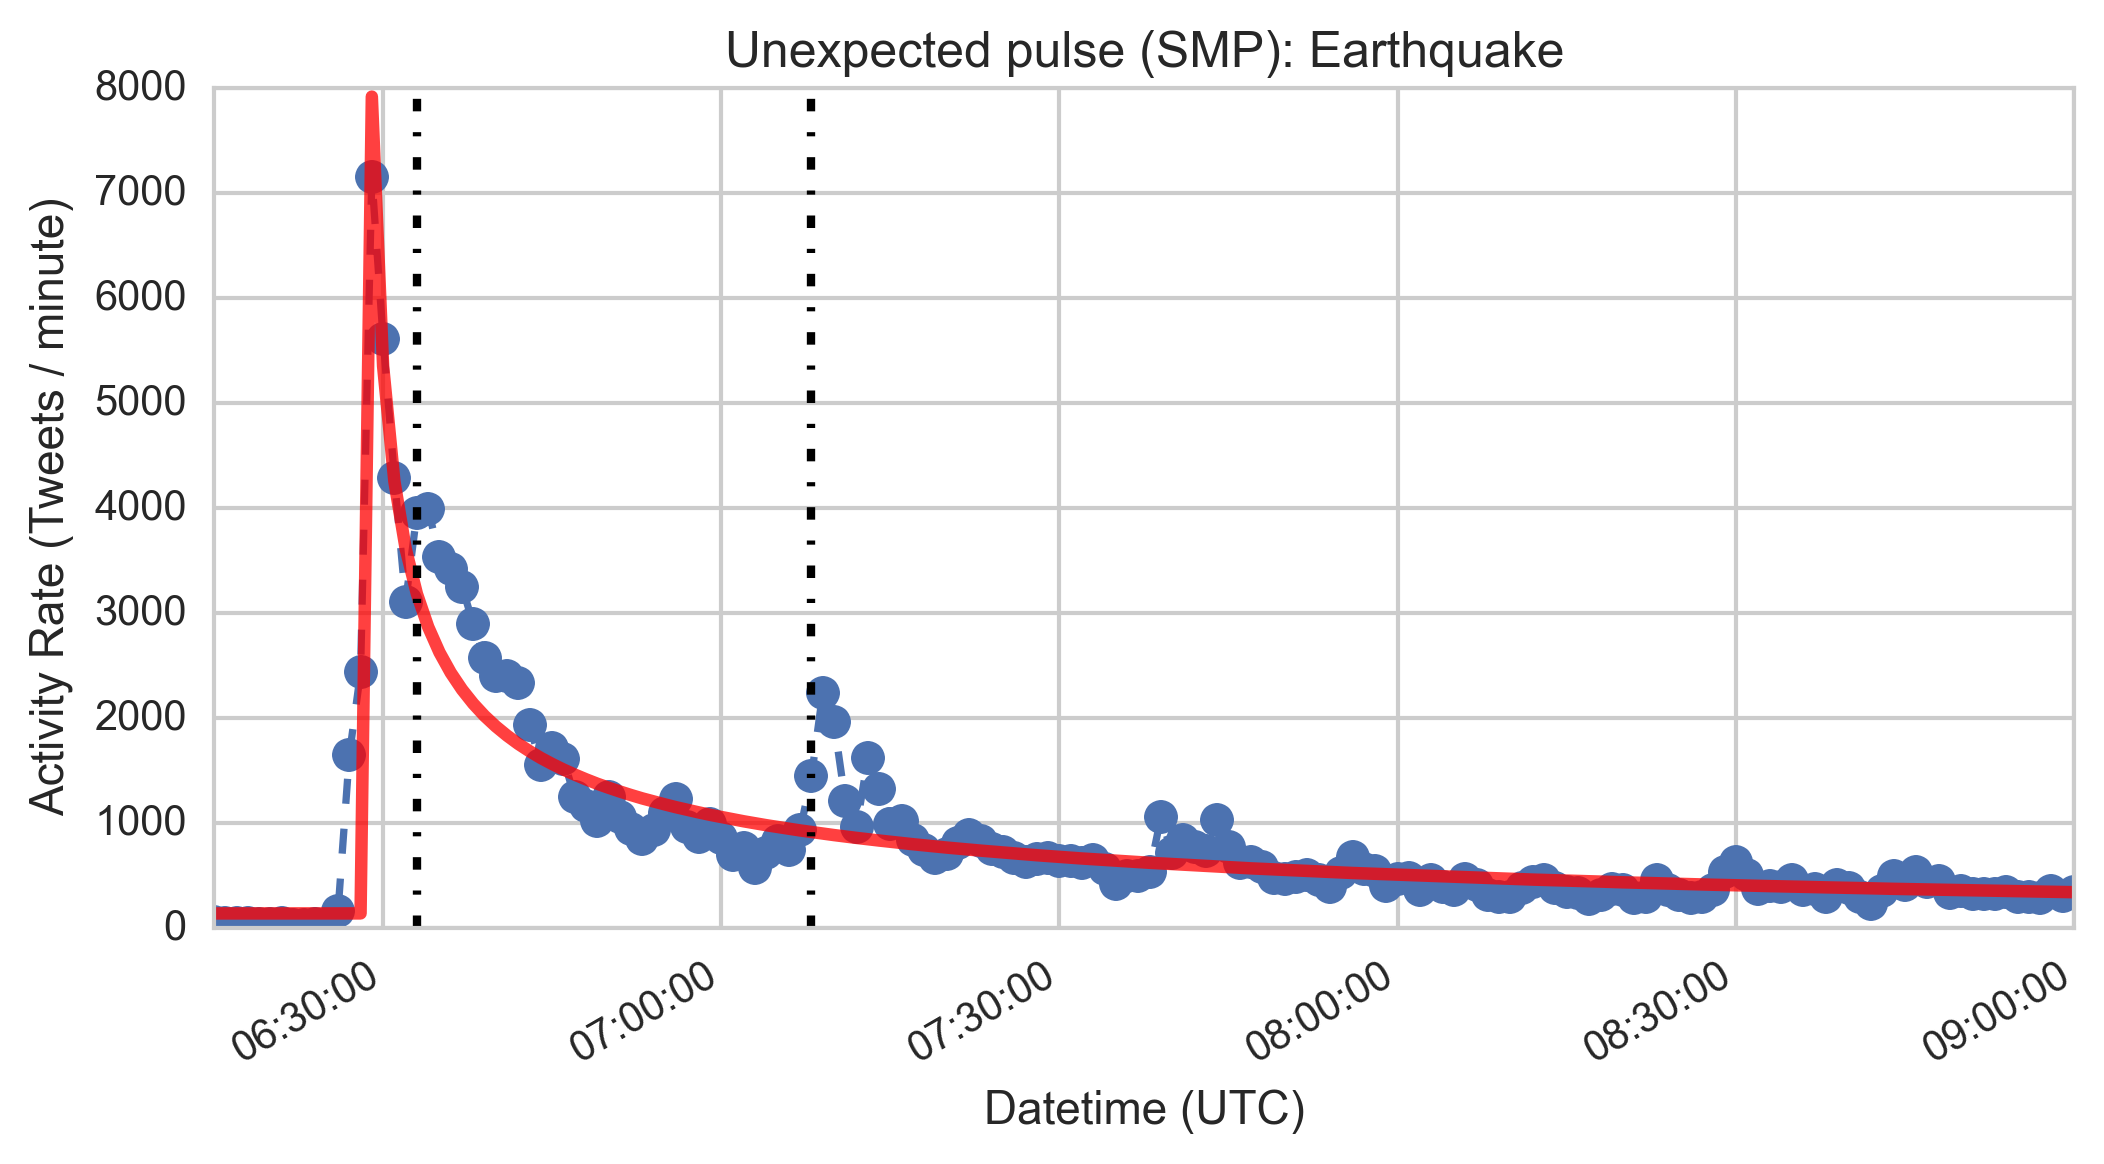
\includegraphics[width=0.9\textwidth]{img/earthquake-deviation.png}
\caption{An SMP associated with an earthquake in April 2016. Within minutes of the SMP peak, the activity rate data shows a spike (dashed, in black) which deviates from the model curve (solid red). A similar spike occurs approximately thirty minutes later (also dashed, in black). Dashed lines connect the data points in the series. This type of deviation can be a valuable signal about changes in the underlying behavior. In this example, we observe a notable increase in the Retweeting of news articles - a different underlying mechanism than that of the SMP. The model can still be fit to a subset of the data -- before the deviation occurs -- to calculate SMP metrics.} 
\label{fig:smp-fit-deviation}
\end{figure}




%%%%%%%%%%%%%%%%%%%%
\section{Conclusion} 
\label{sec:conclusion}

Analysis of Twitter data can provide valuable insight into both events past and those on-going. In this paper, we discussed three types of events that we have observed in the data from the Twitter platform which corresponding to various types of real-world events. While these event types and the Social Media Pulse (SMP) model described in this work represent a relatively simple start, the study and modeling of human behavior on social platforms is a broad and active field of research. 

The observations discussed in this work are not necessarily exclusive to Twitter. But, as a real-time social network the Twitter platform leads to public data which is well-suited for highlighting these kinds of observed behaviors. By applying the tools discussed here, in particular the model for the Social Media Pulse, we can gain quantitative insights into real-time, real-world events, including parametrizing and comparing events. Extensions of this work could include, for example, automated event (or SMP) classification. It is our hope that this work enables the analyst to better quantify their observations and conclusions made from social data streams. 

The latest version of this document and supporting code can be found on GitHub.\cite{pulse} If you find errors or have comments, please email \texttt{shendrickson@twitter.com}. This work is licensed under a Creative Commons Attribution 4.0 International Public License.\cite{CreativeCommons}


% bibliography
% this bib style allows the urls display (ref: http://tex.stackexchange.com/a/133881 )
\bibliographystyle{IEEEtran}      
\bibliography{IEEEabrv,refs-SMP} 

% fin

\includepdf[pages={-}]{back-cover.pdf} 
\end{document}
